\chapter[Metodologia]{Metodologia}

Este capítulo tem como objetivo apresentar a metodologia utilizada para desenvolvimento do trabalho. A seção \ref{met_pesquisa} apresenta a classificação da metodologia utilizada para o desenvolvimento do trabalho, juntamente com o plano metodológico. A seção \ref{met_desenvolvimento} descreve o processo de desenvolvimento utilizado na criação da solução. Por último a seção  \ref{cronograma} apresenta os cronogramas para condução do TCC 1, bem como do TCC 2.
\section{Metodologia de Pesquisa}
\label{met_pesquisa}
Segundo \cite{moresi_metodologia_2003}, a pesquisa pode ser entendida como um conjunto de ações que tem como objetivo encontrar um problema, sendo construída através de procedimentos empíricos e sistemáticos. Para Moresi, existem quatro classificações básicas para a pesquisa, quanto: à natureza, à abordagem, ao objetivo e ao meio pelo qual é feita a investigação. A Figura \ref{img:met_pesquisa} apresenta em quais classificações esse trabalho se baseia.
\graphicspath{{figuras/}}
\begin{figure}[h!]
\centering
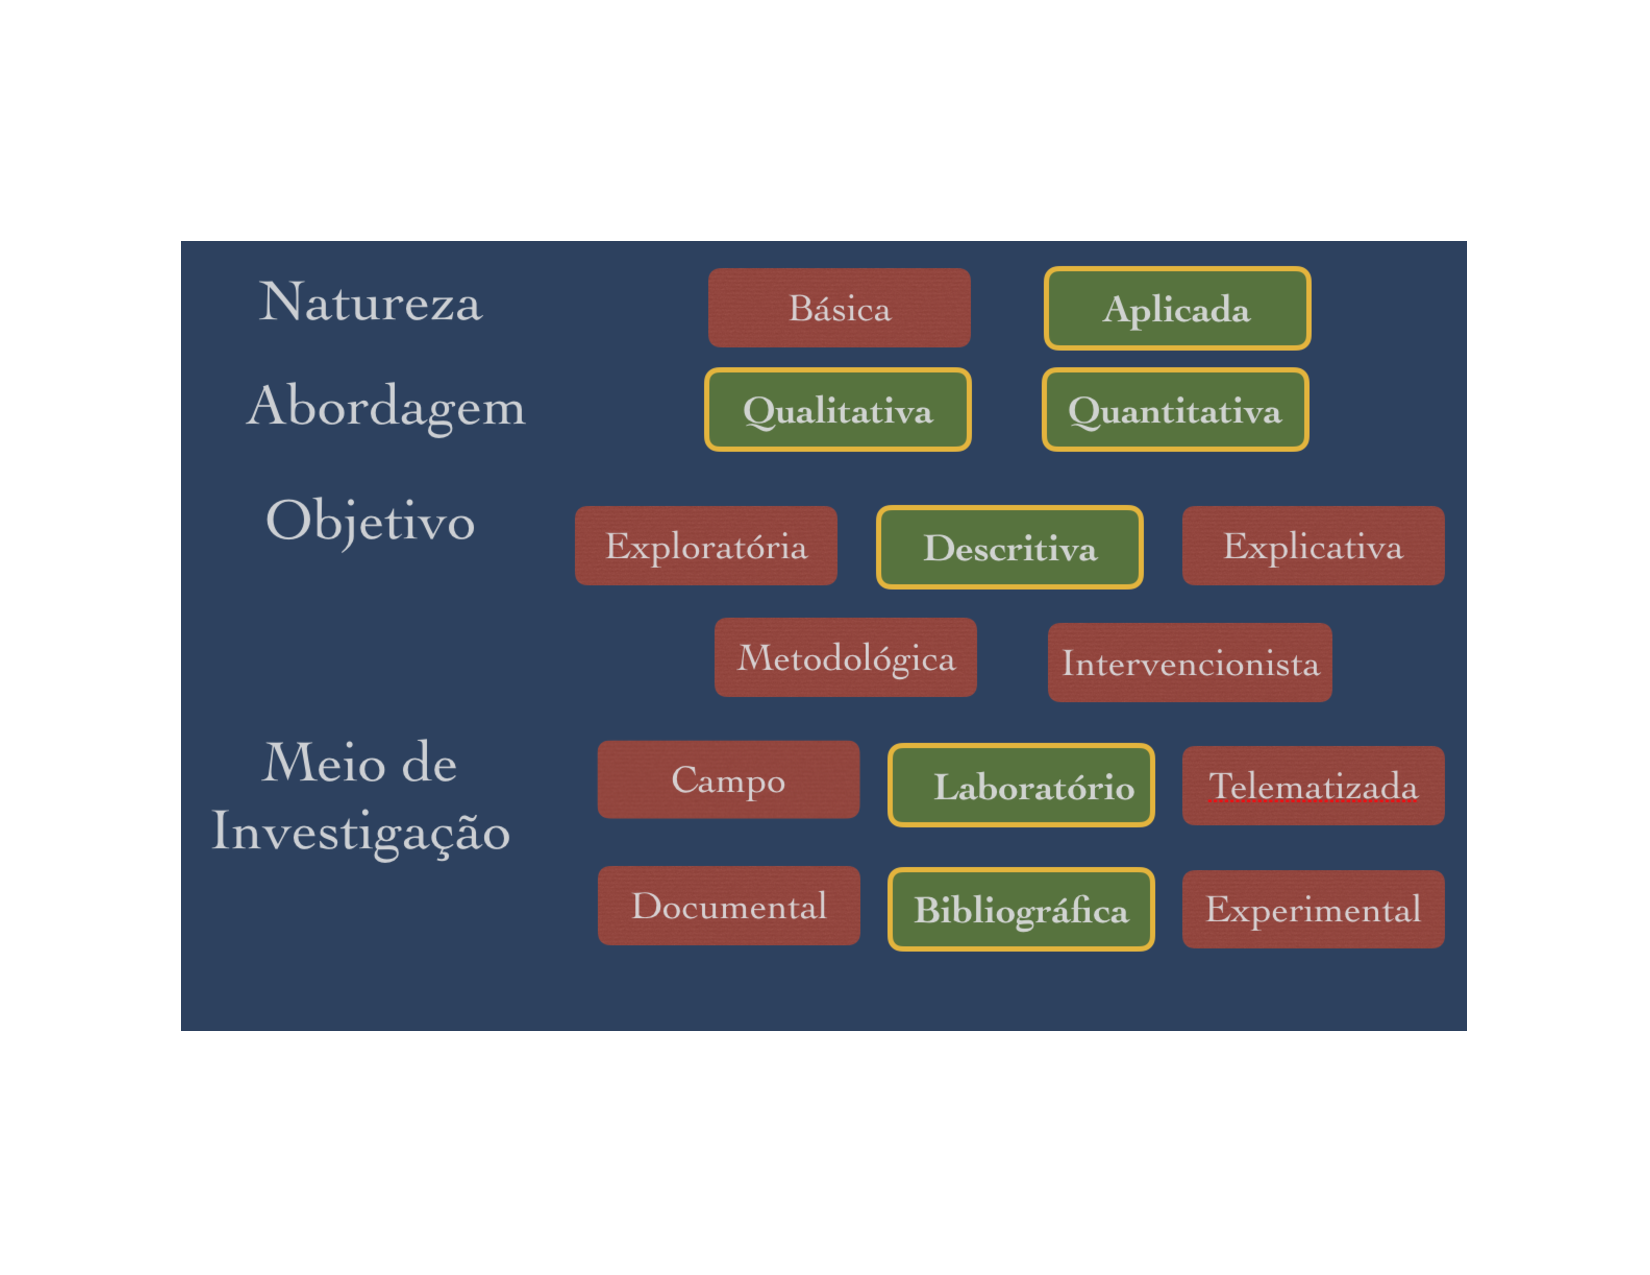
\includegraphics[scale=0.50]{metodologia_pesquisa}
\caption{Seleção das Características Metodológicas. Fonte: \cite{moresi_metodologia_2003}}
\label{img:met_pesquisa}
\end{figure}

Este trabalho tem um caráter mais voltado para  pesquisa aplicada, por envolver características espécificas na contratação de software do Governo Brasileiro. Outra característica que determina este trabalho como pesquisa aplicada é a natureza do trabalho ser voltada para o uso nas áreas de TI dentro dos Órgãos Públicos.

Segundo Tatiana e Denise \cite{tatiana_denise} a pesquisa qualitativa é mais voltada para aspectos da realidade que não podem ser quantificados, mantendo o foco na compreensão. Neste aspecto, o trabalho apresenta características qualitativas. Segundo as autoras \cite{tatiana_denise}, outra característica inerente a este tipo de pesquisa é a observação do mundo social ao mundo natural. Portanto, tal característica apresenta-se de maneira muito forte quando, ao propor a solução, procura-se adotar um conjunto de métricas que são utilizadas no mercado ao invés de outros conjuntos apresentados por outros autores. Oposto à pesquisa qualitativa, os resultados obtidos podem ser quantificados. A pesquisa quantitativa teve como fundamento o pensamento positivista lógico, prima pelas regras da lógica e do raciocínio dedutivo \cite{tatiana_denise}. 

Para Gil \cite{gil_como_2002}, a pesquisa descritiva é focada em analisar características de uma população, fenômeno ou a relação entre as váriaveis que as compõem. Este tipo de pesquisa não visa explicar os fenômenos que estão descrevendo\cite{moresi_metodologia_2003}. Este trabalho apresenta o caráter descritivo ao tratar da natureza das contratações de software para Órgão Públicos Brasileiros, ou quando se fala de um processo de manutenção de software.

Outra característica deste trabalho é a escolha por fazer uma pesquisa de laboratório. Moresi destaca que a pesquisa de laboratório atua em um ambiente controlável, quando o pesquisador não tem a possibilidade de atuar em campo. Neste trabalho, a pesquisa em campo se torna algo complicado, pois é difícil conseguir acesso aos Órgãos Públicos para instalação de uma ferramenta que ainda está em desenvolvimento. Por este motivo, a pesquisa em laboratório é a mais adequada, em que são recriadas as mesmas condições de uma situação em campo, porém, com o controle de um ambiente simulado. Outro meio de pesquisa é a pesquisa bibliográfica. A pesquisa bibliográfica é feita através do aprofundamento de materiais já públicados \cite{tatiana_denise}. Este trabalho também utilizou pesquisa bibliográfica durante a fase de Iniciação, em que o objetivo era estudar propostas similares à definida neste trabalho.

\subsection{Plano Metodológico}
\label{plano_metodologico}
O plano metodológico consiste em duas fases: Iniciação e Execução. Durante o TCC1 será implementada somente a primeira fase. A fase de Execução será implementada no TCC2. A primeira fase (Figura \ref{img:iniciacao}) possui seis atividades principais, são elas: Definir Tema, Validar o Escopo, Elaborar um Roteiro de Pesquisa, Pesquisar Referências, Refinar Pesquisa e Catalogar Material Encontrado.

\graphicspath{{figuras/}}
\begin{figure}
\centering
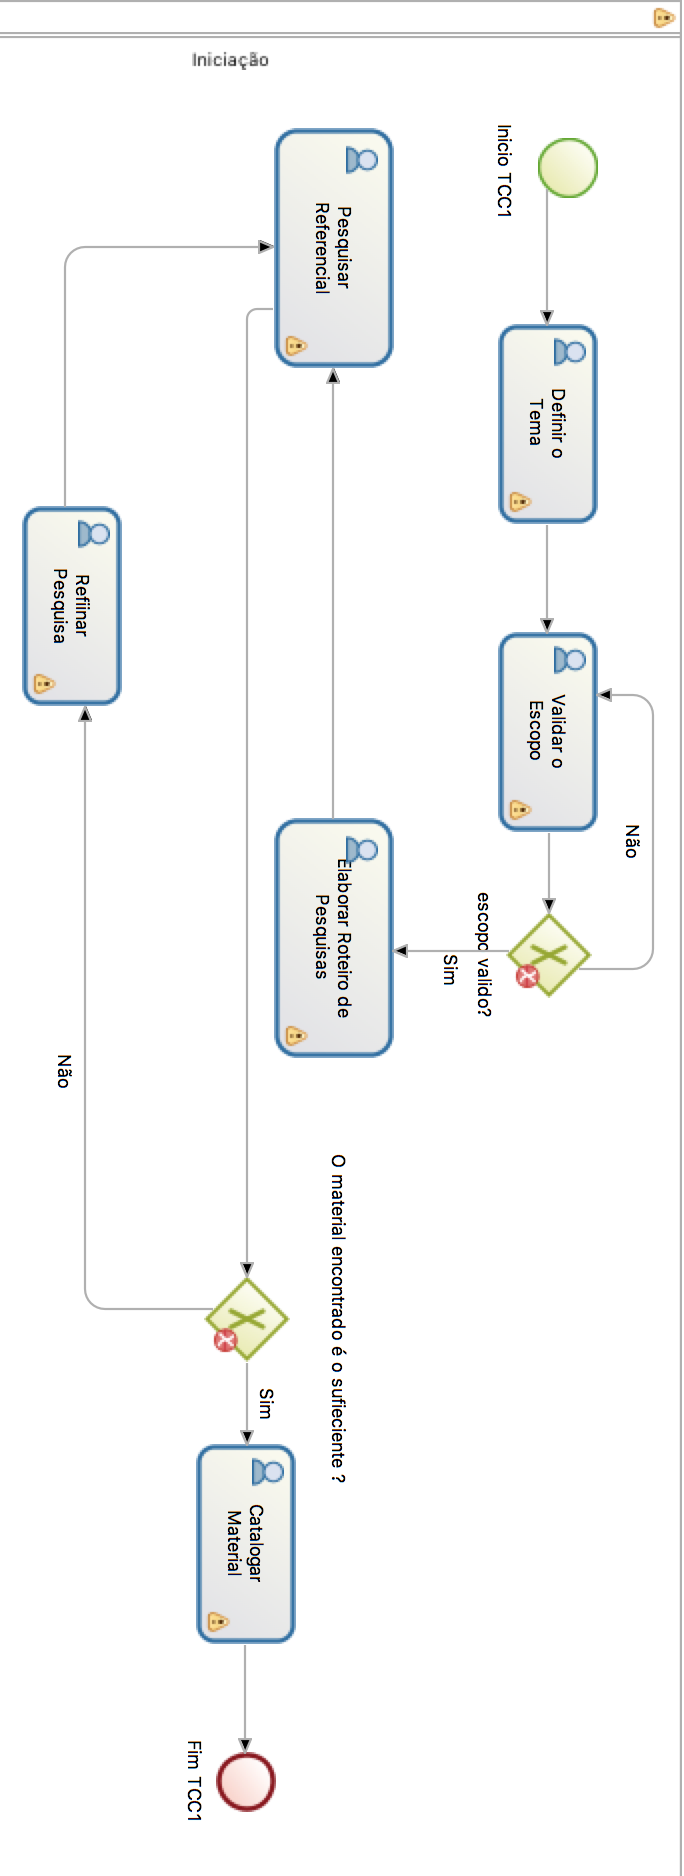
\includegraphics[scale=0.50]{iniciacao}
\caption{Modelagem da Fase de Iniciação}
\label{img:iniciacao}
\end{figure}

A primeira atividade de Definir um Tema acontece logo no início do processo para que seja possível estabelecer em que área e sobre o que será discutido no trabalho. Uma vez escolhido o tema, é preciso definir o escopo do trabalho para que seja possível definir quais são as fronteiras impostas tanto pelo tempo, pois é um prazo curto, quanto pelo conhecimento. Uma vez definido o tema, o escopo é validado juntamente com os professores orientadores para que haja um acordo entre aluno e orientador sobre o que será trabalhado.

Posteriormente, é necessario Elaborar um Roteiro de Pesquisa  que consiste em encontrar a melhor \textit{string}, trabalhando a revisão bibliográfica. Na presente proposta, as \textit{strings} foram montadas de acordo com o tema da pesquisa, portanto, não houve uma string geral que fosse utilizada por todo o processo investigativo. Dessa forma, as primeiras strings foram montadas com base em conceitos chave nos tópicos e áreas de interesse para a presente proposta. Algumas das strings utilizadas inicialmente foram "contratação de software", "criação de um \textit{dashboard}" e "métricas de qualidade". Com o decorrer do trabalho, no processo investigativo, a proposta foi adquirindo um escopo cada vez mais refinado, específico e conciso, culminando na seguinte string de busca final: "utilização de \textit{dashboard} + acompanhamento de métricas + manutenabilidade + Órgão Públicos". 

As atividades de Elaborar Referências e Refinar Pesquisa envolviam o processo de aplicar a \textit{string} nos motores de busca selecionados, que no caso foram Google Scholar e Periódicos Capes. Uma vez aplicada a \textit{string}, o primeiro ponto a ser observado nos resultados era o título do material. Caso o título tivesse alguma relação com o tema pesquisado, o artigo era separado (esse processo era válido somente para as duas primeiras páginas de resultados). Com os artigos separados lia-se os tópicos do artigo, e havendo um conteúdo referente à pesquisa, lia-se o artigo completo. Caso o  material encontrado não atendesse à temática do trabalho, gerava-se uma nova \textit{string} de busca com termos aproximados ou mais refinados e o processo se repetia.

Catalogar Material é uma atividade focada em guardar os materiais encontrados colocando uma  \textit{tag} referente ao tema a que o artigo se refere e uma breve descrição sobre os principais pontos do material. Esse armazenamento é feito através de duas ferramentas de gerenciamento bibliográfico, o Zotero e o BibDesk. O Zotero foi utilizado para fazer a catalogação \textit{online} dos materiais, e gerar a bibliografia encontrada de cada material conforme ilustra a Figura \ref{img:zotero}.

\graphicspath{{figuras/}}
\begin{figure}[H]
\centering
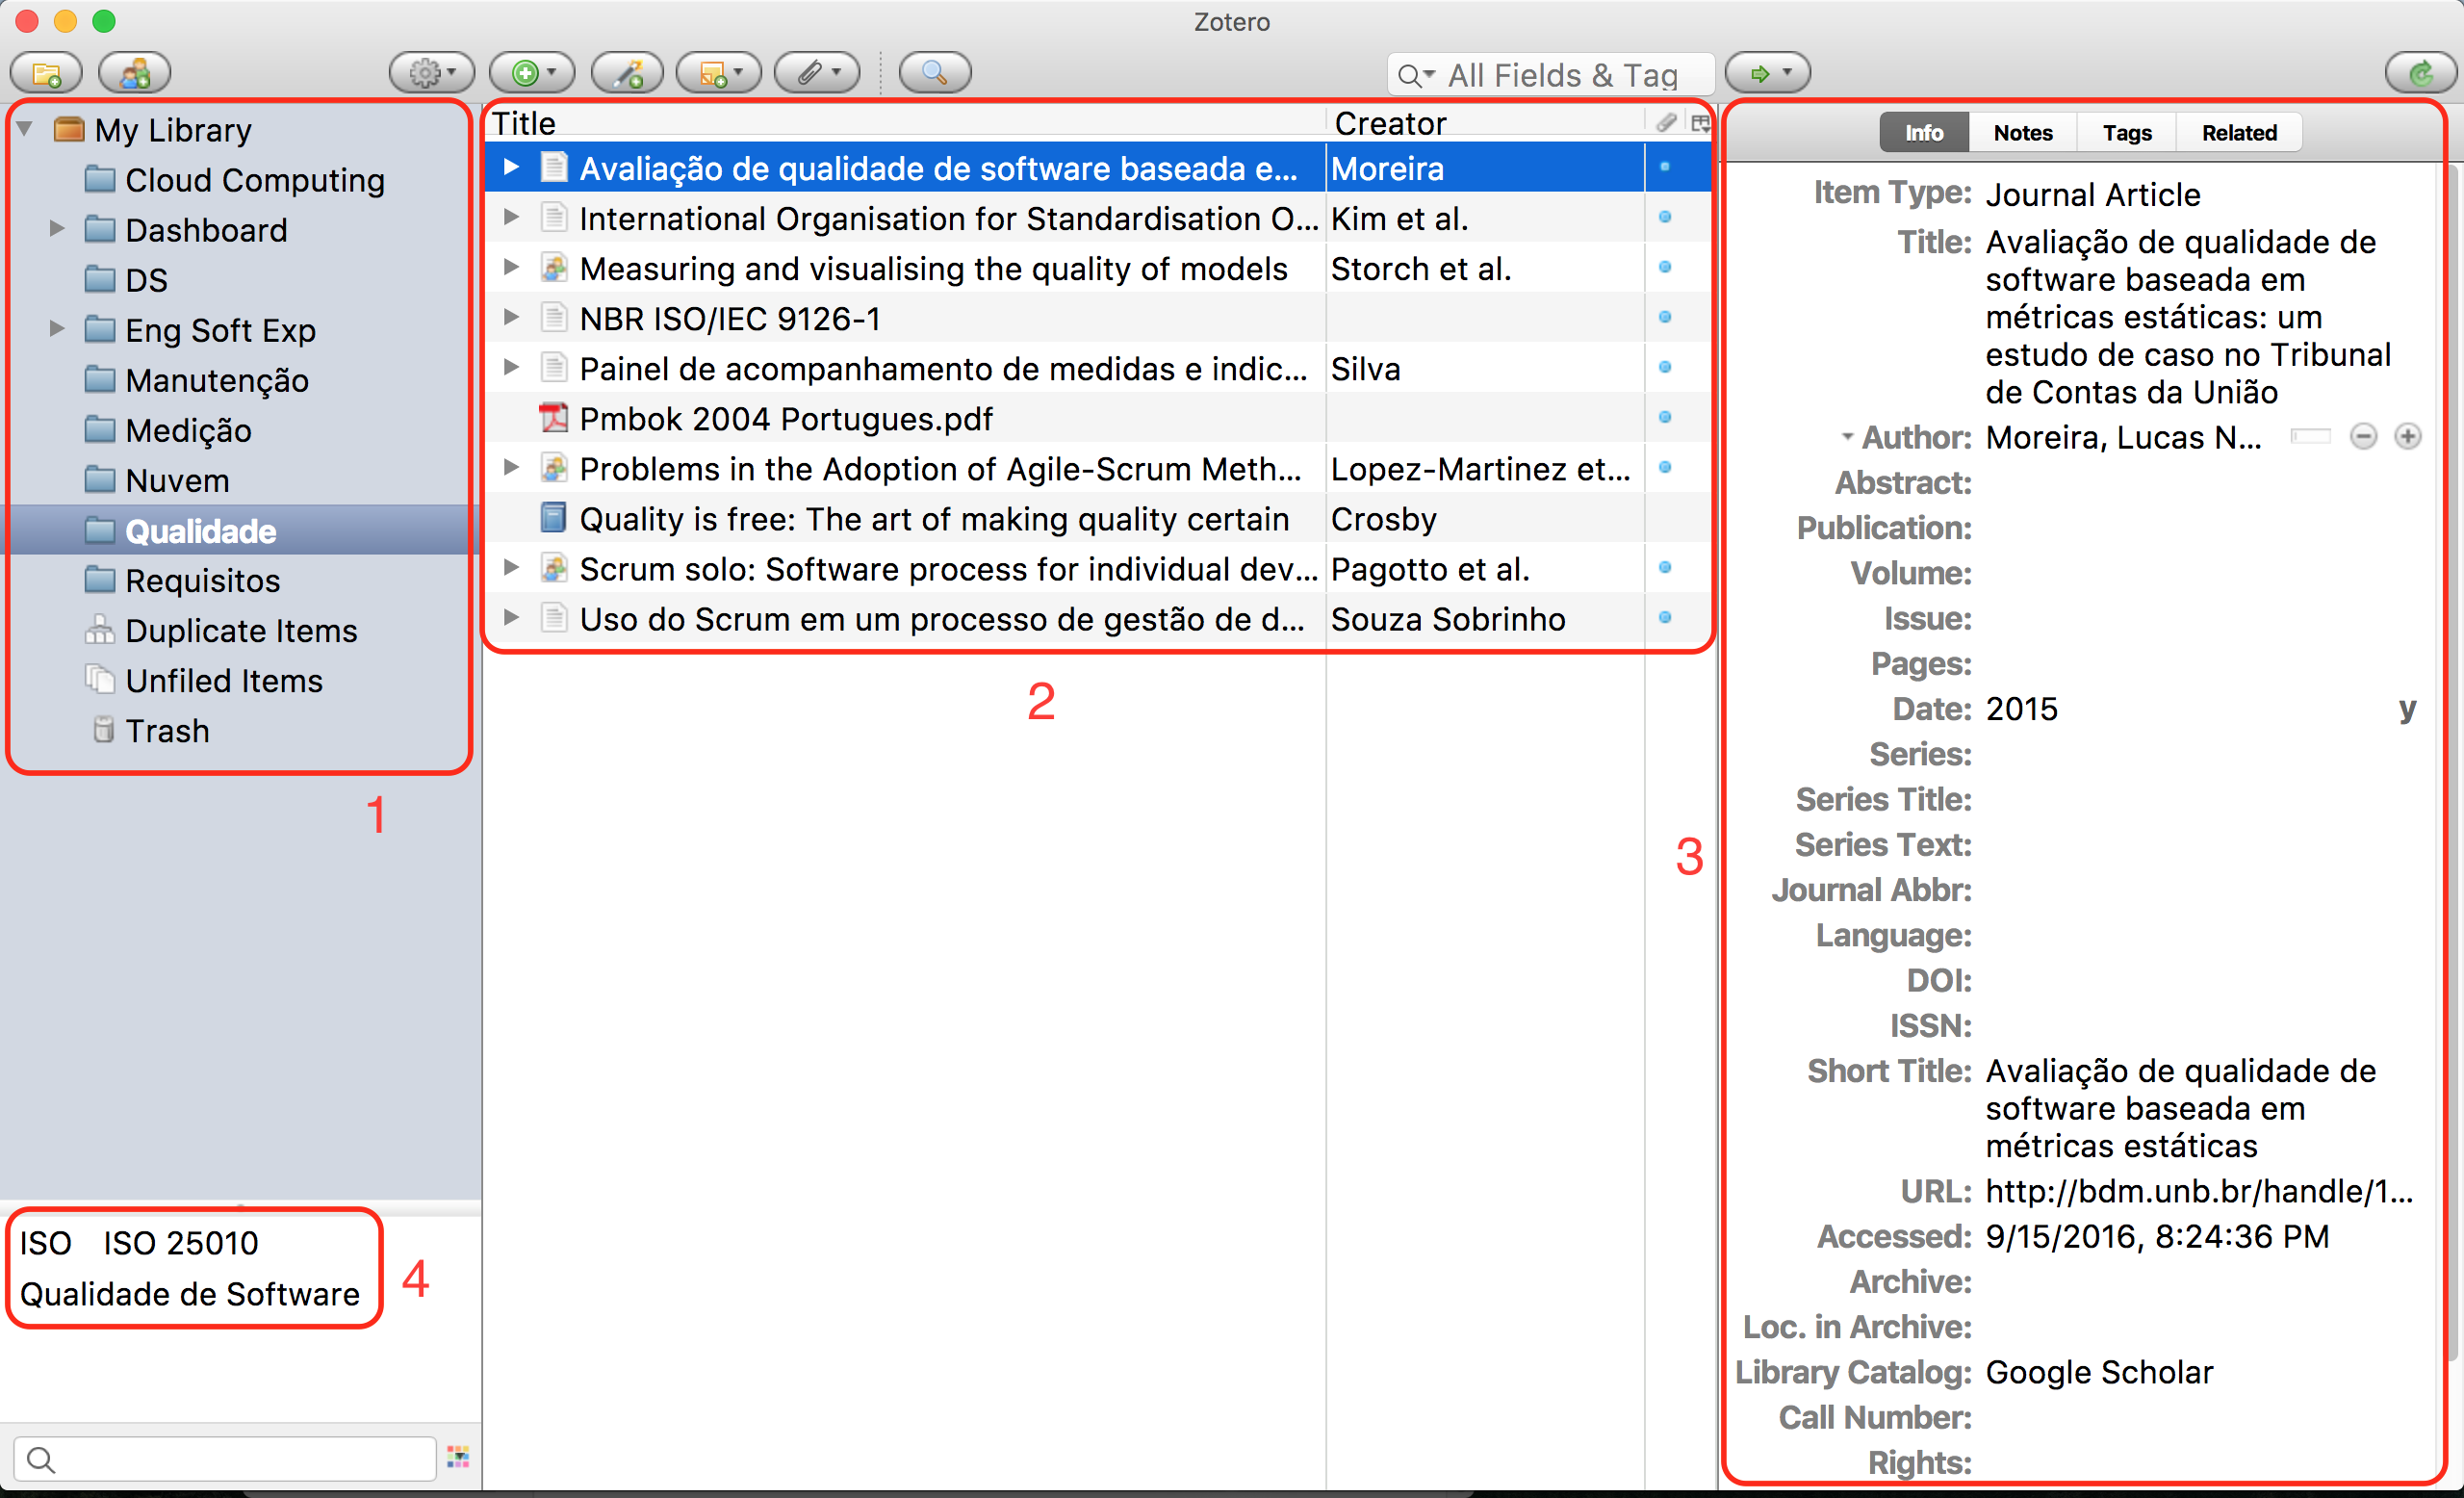
\includegraphics[scale=0.40]{zotero_edit2.png}
\caption{\textit{Screenshot} do Zotero contendo as categorias dos materiais pesquisados, suas \textit{tags} e anotações}
\label{img:zotero}
\end{figure}

\begin{itemize}
\item Área 1 - Categorização por pastas dos artigos encontrados.
\item Área 2 - Artigos referentes à categoria selecionada. Dentro de cada artigo, é possível encontrar a nota e um \textit{link} para leitura do artigo selecionado.
\item Área 3 - Informações do artigo selecionado.
\item Área 4 - \textit{Tags} referentes ao artigo.
\end{itemize}
Uma vez que o material era catalogado no Zotero, o mesmo era exportado para o Bibdesk por ter uma melhor integração com o Latex.

Após catalogar o material encontrado, finaliza-se a fase de iniciação do projeto. Esta fase deixa como insumo para a próxima fase, o trabalho produzido até então, e decisões de escopo e cenários de uso que serão implentados na Fase de Execução. 

A Fase de Execução (Figura \ref{img:execucao}) possui sete atividades, sendo que a atividade de Documentação ocorre durante todo o processo. O objetivo desta fase é implementar o que foi decidido na Fase de Iniciação. A primeira atividade da segunda fase é Analisar o Ambiente. Por se tratar de um ambiente simulado, é necessário que se estude quais são as melhores ferramentas e a configuração entre elas para que se reproduza um ambiente mais próximo do real possível. Uma vez definido, é necessário Configurar este ambiente  o que deve ser feito orientando-se pelas configurações de um ambiente real.

\graphicspath{{figuras/}}
\begin{figure}
\centering
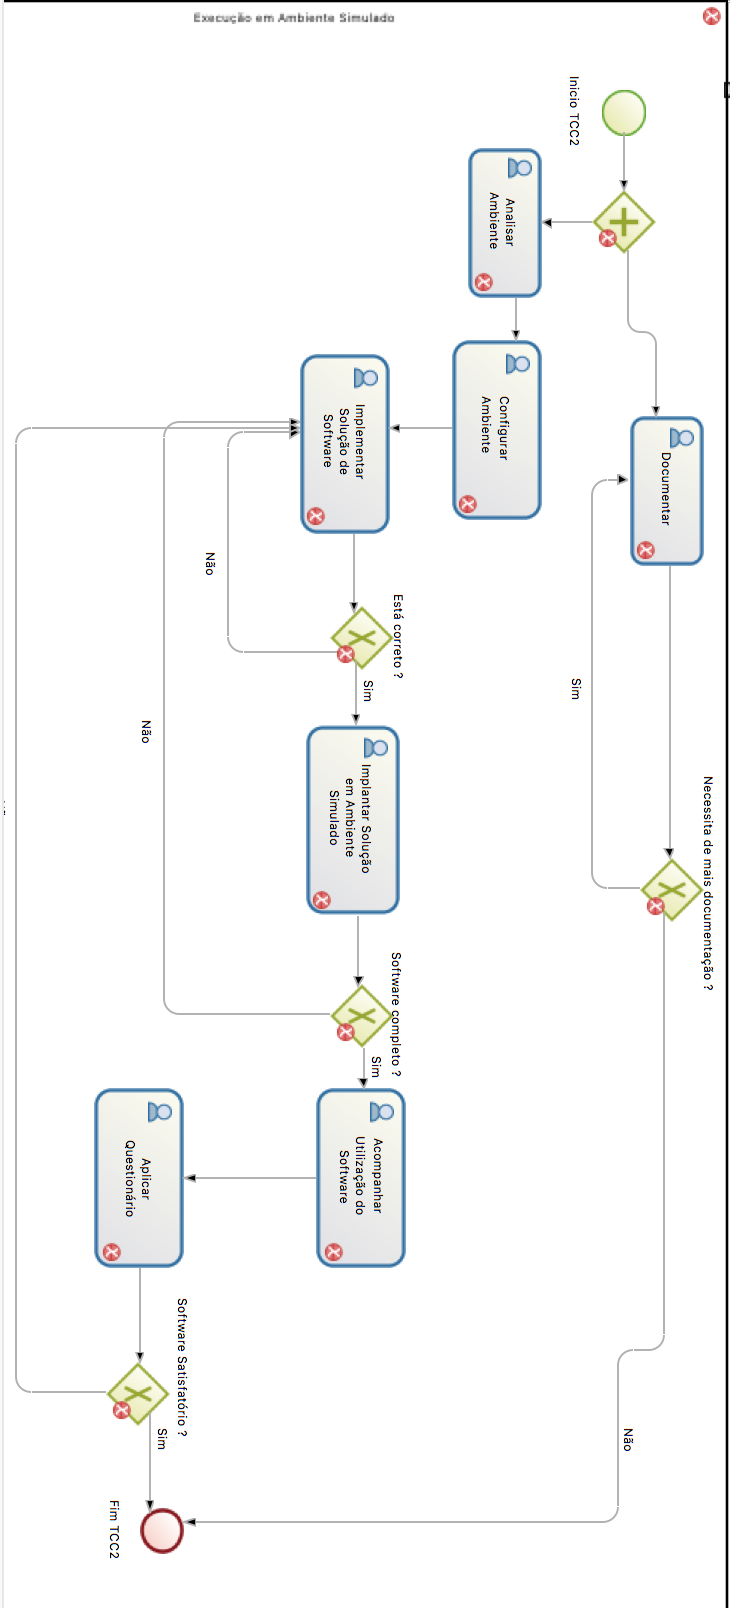
\includegraphics[scale=0.60]{execucao}
\caption{Modelagem da Fase de Execução}
\label{img:execucao}
\end{figure}

A terceira atividade é Implementar a Solução. Esta atividade segue os princípios de desenvolvimento ágil para construção de soluções em software. Para isso, seu desenvolvimento é feito de maneira iterativa incremental de forma que a cada iteração ocorra um implemento funcional de software. Ao fim de cada iteração, se o software produzido estiver funcionando e testado, ele é colocado no ambiente simulado, equivalente a um ambiente de produção, para que se possa acompanhar o seu funcionamento.

Uma vez que a solução esteja pronta para uso,  esta será disponibilizada para um conjunto de utilizadores que irão testar a solução bem como documentar as suas impressões quanto à utilização da solução. A última atividade desta fase é relacionada ao questionário que é aplicado aos utilizadores da ferramenta para que se possa avaliar o quão pertinente e adequada foi a solução. 

Com a Fase de Execução finalizada, encerra-se o processo. Nesta segunda fase, os principais artefatos são: a solução funcionando e um refinamento do documento entregue na primeira fase. A Modelagem completa do processo encontra-se no Anexo 5 deste documento.


\section{Metodologia de Desenvolvimento}
\label{met_desenvolvimento}
O \textit{dashboard} será criado utilizando uma adaptação da metodologia de desenvolvimento Scrum \cite{pagotto_scrum_2016}. O Scrum é uma metodologia de desenvolvimento de software baseada em princípios de desenvolvimento ágil. As metodologias ágeis ganharam popularidade por serem adaptáveis a 	times pequenos, ou projetos que possuam prazos curtos na entrega do software, e ainda projetos com requisitos constantemente alterados \cite{lopez-martinez_problems_2016}. Como o Scrum é um modelo de desenvolvimento iterativo e incremental, propõe que o projeto de desenvolvimento seja estruturado em pequenas entregas, chamadas de \textit{sprints}. Essas \textit{sprints} podem ser associadas a pequenos ciclos de desenvolvimento, os quais duram entre duas a quatro semanas. As \textit{sprints} são consecutivas e, nesse período, algumas funcionalidades do sistema são implementadas e testadas \cite{pagotto_scrum_2016}. Na Figura \ref{img:scrum} pode-se observar que as funcionalidades desenvolvidas na \textit{sprint} advêm de um escopo definido no início do projeto,  chamado de \textit{product backlog}, que é o conjunto de todas as funcionalidades do sistema. O conjunto de funcionalidades separadas para uma determinada \textit{sprint} é chamada de \textit{sprint backlog}\cite{sabbagh_scrum:_2014}.
\graphicspath{{figuras/}}
\begin{figure}[H]
\centering
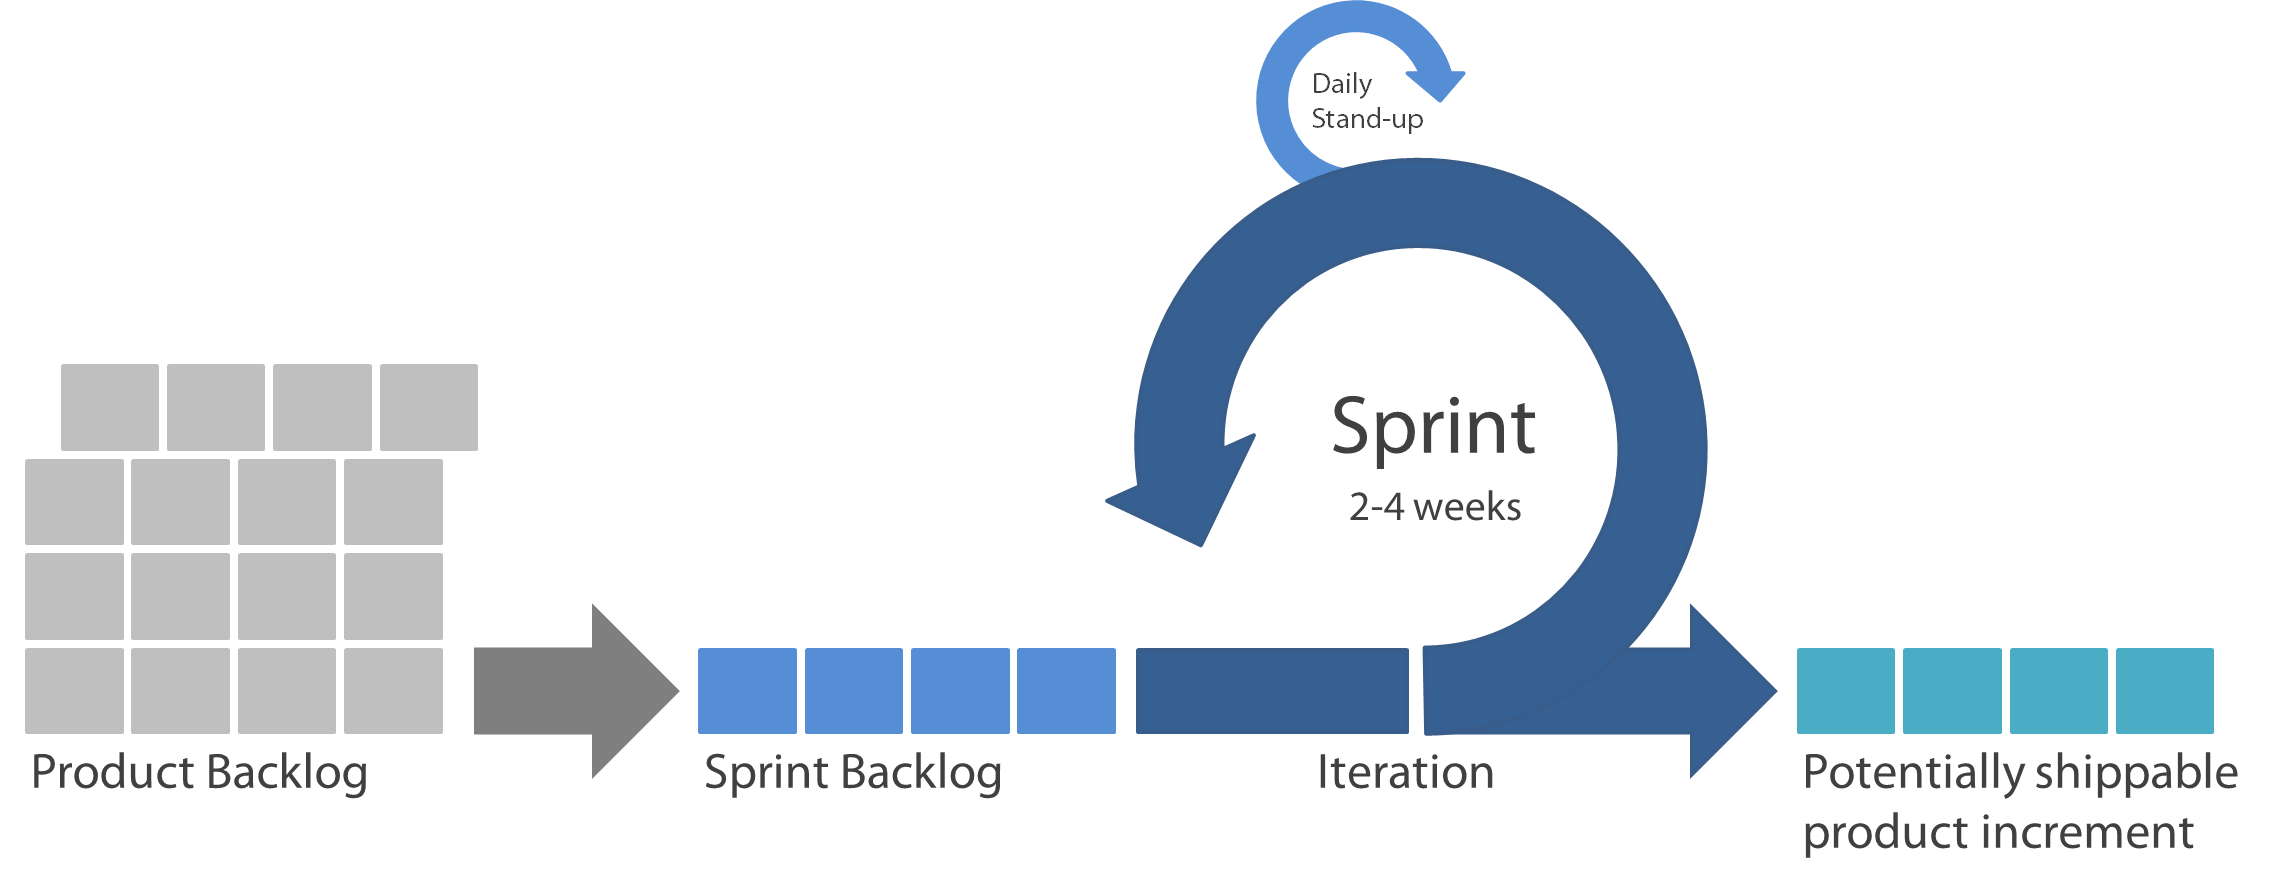
\includegraphics[scale=0.40]{scrum}
\caption{Ciclo de Desenvolvimento do Scrum}
\label{img:scrum}
\end{figure}

Os principais conceitos que foram utilizados da metodologia foram:
\begin{itemize}
\item \textit{\textbf{Product Backlog}}: Lista de atividades que representam as funcionalidades que serão construídas no projeto. O \textit{product owner} é quem escreve o \textit{product backlog}. Essas atividades são mutáveis ao decorrer do projeto, pois a equipe de desenvolvimento acaba conhecendo mais do produto \cite{sabbagh_scrum:_2014}.
\item \textit{\textbf{Sprint}}: Ciclo de desenvolvimento com prazo definido em que são desenvolvidas as atividades do projeto. Neste trabalho, definiu-se como sendo 15 dias o período referente a uma \textit{Sprint}
\item \textit{\textbf{Sprint Backlog}}: Atividades referentes à uma determinada \textit{Sprint}, na qual a equipe de desenvolvimento se compromete a entregar. Estas atividades são retiradas do \textit{product backlog} \cite{mahnic_case_2011}.
\item \textbf{\textit{User Story}}: Descrição do ponto de vista do usuário sobre uma funcionalidade do produto. Este artefato é composto do que é conhecido como 3C's, Cartão, Conversa e Confirmação. O cartão é referente ao fato de se documentar a conversa em um cartão, este sendo acessível a todo o time de desenvolvimento. A conversa é uma breve descrição da funcionalidade sob o olhar do usuário. Um exemplo pode ser observado na Figura \ref{img:us}. A confirmação ou critérios de aceitação é um \textit{checklist} abordando o que deve ser verificado para que a história seja dada como concluída.
\graphicspath{{figuras/}}
\begin{figure}[H]
\centering
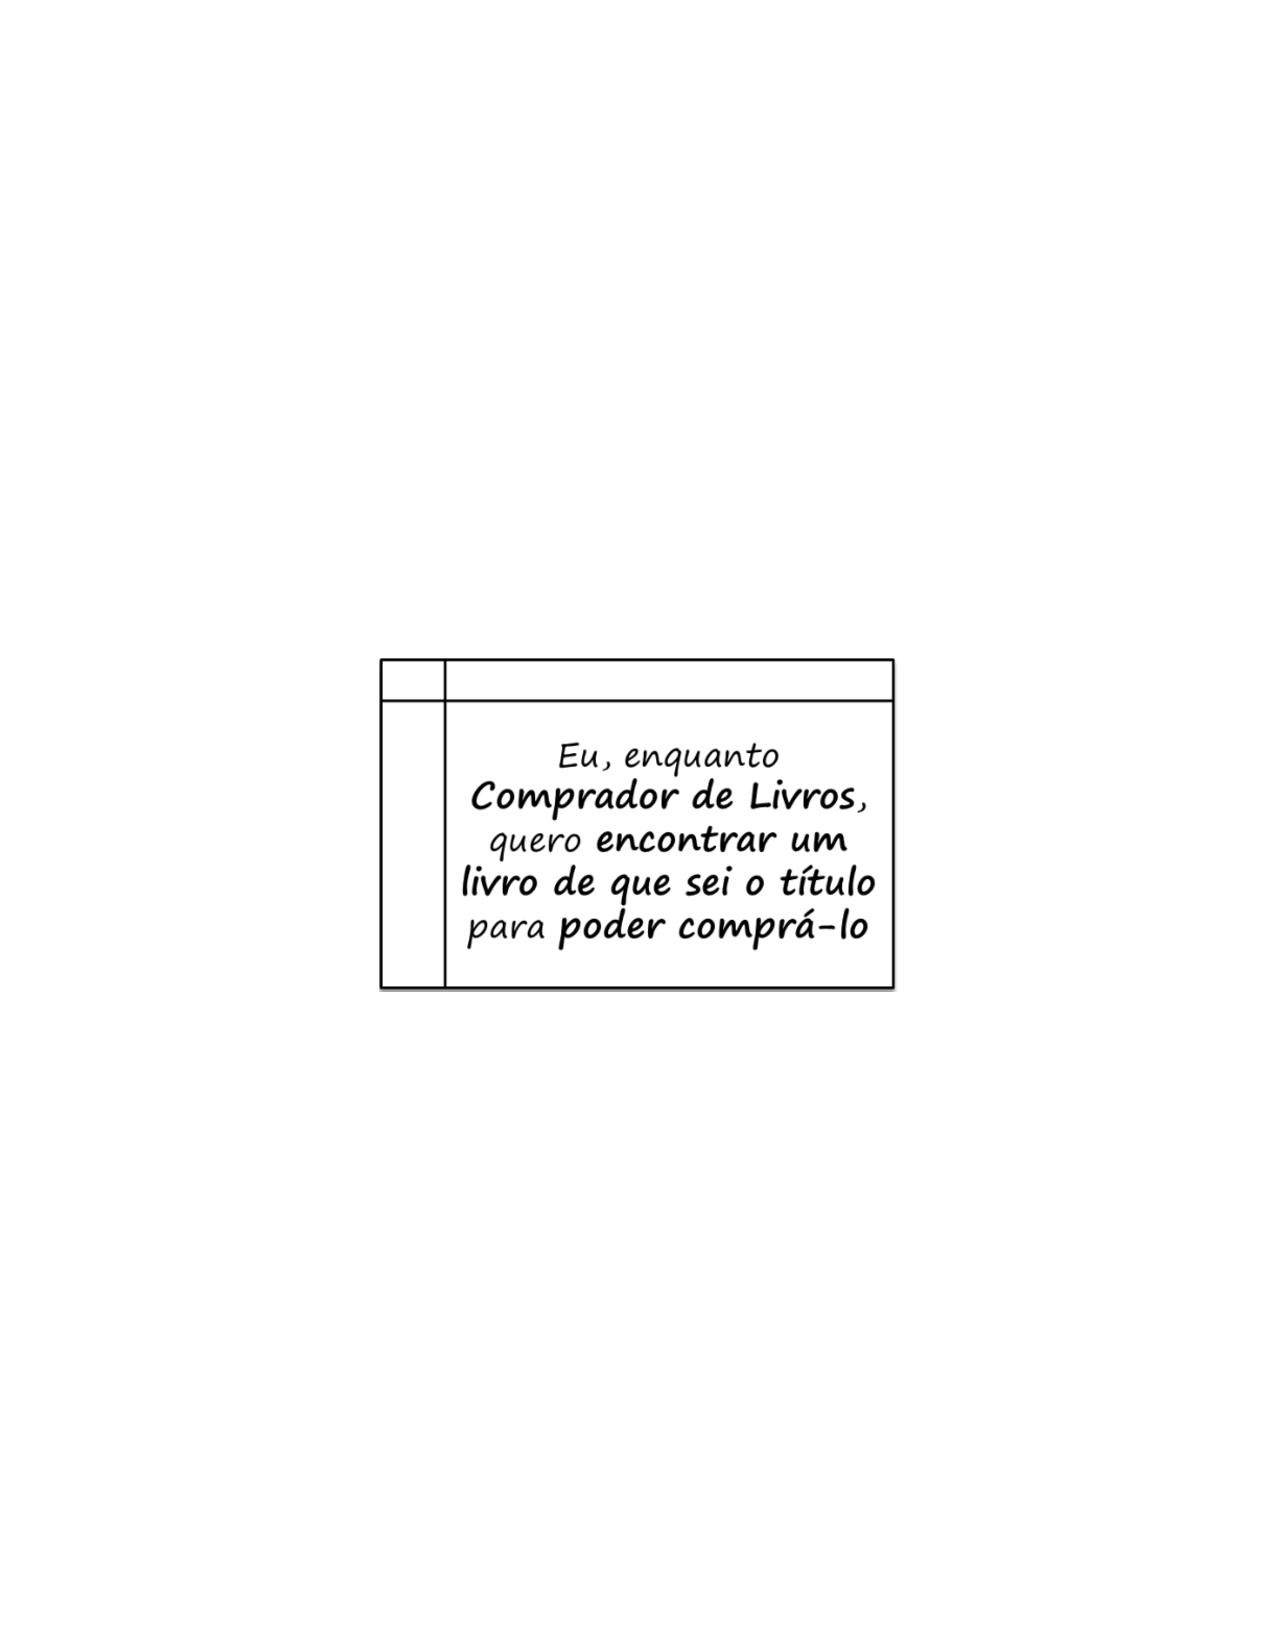
\includegraphics[scale=0.80]{US}
\caption{Exemplo de História de Usuário. Fonte: \cite{sabbagh_scrum:_2014}}
\label{img:us}
\end{figure}
\item \textit{\textbf{Story Point}}:Unidade relativa que caracteriza o esforço da equipe de desenvolvimento para finalizar uma atividade. A escala utilizada é definida pela equipe de desenvolvimento. Neste trabalho, será utilizado a escala de Fibonacci (1,2,3,5,8,13, ...). 
\item \textit{\textbf{Kanban}}: Forma de visualização de atividades muito utilizadas com cartões, os quais são movimentados em um quadro determinando o status da atividade, conforme mostra a Figura \ref{img:kanban}.
\graphicspath{{figuras/}}
\begin{figure}[H]
\centering
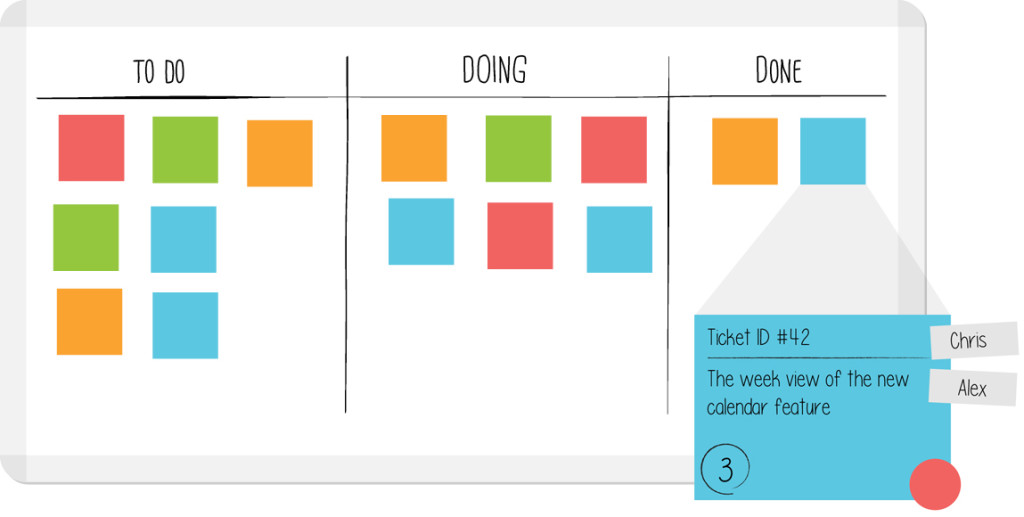
\includegraphics[scale=0.40]{kanban}
\caption{Exemplo de \textit{Kanban}}
\label{img:kanban}
\end{figure}

\end{itemize}

Por se tratar de uma adaptação do Scrum, algumas modificações foram necessárias para que a metodologia possa atender às necessidades do trabalho. Uma das alterações que foram feitas é quanto ao time de desenvolvimento. Para este projeto o time de desenvolvimento será de uma pessoa, diferente do Scrum tradicional, que define a quantidade de membros em um time de desenvolvimento deve ser entre 3 a 9 pessoas \cite{sabbagh_scrum:_2014}. Outra adaptação, é quanto ao \textit{Product Owner}(P.O) que no Scrum tradicional tem o papel de garantir o retorno do investimento para os \textit{stakeholders}. Nesse trabalho o papel de P.O será realizado pelo Orientador deste trabalho. No papel de cliente, será utilizado os próprios usuários que realizarão a avaliação da solução.


\section{Cronograma}
\label{cronograma}

Para que se possa ter uma visão mais abrangente da organização do trabalho, foi criado um cronograma em que constam as atividades definidas no \ref{plano_metodologico}. Este cronograma serve como orientação ao desenvolvimento e planejamento do projeto. Contudo, com o decorrer das atividades, este artefato poderá sofrer alterações. O cronograma foi dividido em duas tabelas (Tabela \ref{cronograma_tcc1} e Tabela \ref{cronograma_tcc2}) referentes às atividades do TCC1 e TCC2 respectivamente.

\subsection{Cronograma TCC1}
A Tabela \ref{cronograma_tcc1} apresenta um cronograma em relação às ativdades a serem desenvolvidas enquanto TCC1.

\begin{table}[h!]
\centering
\caption{Cronograma TCC1}
\label{cronograma_tcc1}
\begin{tabular}{lllll}
\textbf{Atividade}           & \textbf{Agosto} & \textbf{Setembro} & \textbf{Outubro} & \textbf{Novembro} \\ \hline
Definir Tema                 & X               &                   &                  &                   \\ \hline
Validar Escopo               & X               &                   &                  &                   \\ \hline
Elaborar Roteiro de Pesquisa &                 & X                 & X                &                   \\ \hline
Pesquisar Referência         &                 &                   & X                & X                 \\ \hline
Refinar Pesquisa             &                 &                   & X                & X                 \\ \hline
Catalogar Material           &                 &                   &                  & X                 \\ \hline
\end{tabular}
\end{table}

\subsection{Cronograma TCC2}
A Tabela \ref{cronograma_tcc2} apresenta um cronograma em relação às ativdades a serem desenvolvidas enquanto TCC2.
\begin{table}[h!]
\centering
\caption{Cronograma TCC2}
\label{cronograma_tcc2}
\begin{tabular}{lllll}
\textbf{Atividade}                     & \textbf{Março} & \textbf{Abril} & \textbf{Maio} & \textbf{Junho} \\ \hline
Documentar                             & X              & X              & X             & X              \\ \hline
Analisar Ambiente                      & X              &                &               &                \\ \hline
Configurar Ambiente                    & X              &                &               &                \\ \hline
Implementar Solução de Software        &                & X              & X             &                \\ \hline
Implantar Solução em Ambiente Simulado &                & X              & X             &                \\ \hline
Acompanhar Utilização do Software      &                &                &               & X              \\ \hline
Aplicar Questionário                   &                &                &               & X              \\ \hline
\end{tabular}
\end{table}

\section{Resumo do Capítulo}
A pesquisa pode ser classificada de diversas formas. Neste a projeto, a natureza da pesquisa pode ser classificada como Aplicada, devido ao uso específico nas áreas de TI, para uma situação específica que é a contratação de software. Quanto à abordagem, a pesquisa é Hibrida, pois existe momentos em que a pesquisa assume um caráter Qualitativo (forma de se analisar e coletar os dados é feita de maneira empírica), contudo, existe um lado Quantitativo na pesquisa (ao que se refere à pesquisa que é feita com o possíveis usuários). Quanto ao objetivo, essa pesquisa tem um caráter Descritivo, pois observa fatores de um grupo e os descreve neste caso a maneira como funciona a aquisição de software por parte da APF. E, por último, quanto ao meio de investigação que é Laboratorial e Bibliográfico. Laboratorial pois, todo o desenvolvimento da pesquisa é feita em um ambiente controlado e não em campo, e Bibliográfico, pois foi feito um levantamento bibliográfico durante a primeira fase do projeto.

Quanto à metodologia de desenvolvimento, optou-se por uma adaptação da metodologia Scrum. Tal escolha deu-se pelo fato de que o framework da metodologia é adaptável para times de desenvolvimento pequenos e com entregas de produtos de software em curtos períodos de tempo.
